\documentclass[12pt]{article}
\usepackage[top=1cm, bottom=2cm, left=2cm, right=2cm]{geometry} 
%\usepackage{amssymb} %maths
\usepackage{amsmath} %maths
\usepackage{graphicx}
\usepackage{xspace}
\usepackage{perpage}
%
\renewcommand*{\thefootnote}{\fnsymbol{footnote}}
\MakePerPage{footnote}

\renewcommand{\c}{\textit{c.}\xspace}
\newcommand{\eg}{\textit{e.g.}\xspace}
\newcommand{\etc}{\textit{etc.}\xspace}
\newcommand{\ie}{\textit{i.e.}\xspace}
\newcommand{\Nb}{\textit{N.b.}\xspace}
\newcommand{\nb}{\textit{n.b.}\xspace}
\newcommand{\xb}{{\boldsymbol x}}

\newcommand{\Flat}{{\cal F}}
\newcommand{\screen}{{\cal I}}
\newcommand{\additive}{{\cal A}}
\newcommand{\qe}{{\cal S}}

\newcommand{\TBD}{\textit{T.B.D.}\xspace}
\newcommand{\XXX}[1]{\textbf{XXX #1}\xspace}

\begin{document}
\title{DM's Plans for Calibrated Photometry}
\author{Robert Lupton and Mario Juri\'c}
%\date{1996-03-06}
\maketitle
\tableofcontents

\section{Introduction}

In the notation defined in
``Level 2 Photometric Calibration for the LSST Survey'' (Lynne Jones; LSE-180)
the number of detected counts $C_{nat, b}$ from an astronomical source with flux
$F_\nu$ in time $\Delta t$ in band $b$ is
$$
C_{nat, b} = \frac{\pi D^2 \Delta t}{4 g h} \int_0^\infty F_\nu(\lambda)
                                                   S^{atm}(\lambda) S_b^{sys}(\lambda) \,d\lambda/\lambda
$$
where $D$ is the telescope's effective diameter, $g$ the gain (photoelectrons per DN),
and $h$ Planck's constant.

We are interested in $S^{atm}$ and $S_b^{sys}$, the probabilities of a photon passing through 
the atmosphere and telescope/camera (including the mirrors, filter, and lenses) and being detected.  We shall
also need $S_{b, std}$, which we shall choose to be close to an average $S^{atm} S_b^{sys}$.

Our task is, of course, to estimate $C_{std, b} \equiv \int_0^\infty F_\nu S_{b, std} \,d\lambda/\lambda$
given $C_{nat, b}$; doing this correctly requires knowledge of the object's SED.

Measuring $C_{std, b}$ splits into a number of separate operations, and we need to estimate:
\begin{itemize}
\item
  the instrumental sensitivity $S_b^{sys}(\lambda, \xb)$
\item
  the atmospheric transmissivity $S^{atm}(\lambda)$
\item
  the telescope (including optics and filters)
\item
  the detector efficiencies
\item
  the object's SED
\item
  the background level and $C_{std, b}$
\end{itemize}

\section{The instrumental sensitivity $S_b^{sys}(\lambda, \xb)$}
\label{secInstrumental}

We will use a number of data sets to measure the \textit{in situ} sensitivity:
\begin{itemize}
  \item Broad-band flats
  \item ``Monochromatic'' (\c 1nm bandwidth) flats, calibrated with NIST photodiodes observing the calibration screen.
  \item A set of spots from the Stubbs Projector\footnote{
    A source of collimated monochromatic light, driven by a light source equivalent to that used to illuminate
    the flatfield screen, capable of generating a focused spot on the focal plane.  }
\end{itemize}

Let $\screen(\lambda, \xb)$ be the illumination of the focal plane due to the illuminated flatfield screen;
we know the wavelength dependence of the screen illumination from the NIST diode data.

One might hope that $\screen$ would be a function only of $\lambda$ and the flatfield image $\Flat_b(\lambda,
\xb)$ would simply be to $\screen(\lambda)\,S_b^{sys}$; unfortunately your hopes are unfounded.

Non-uniform illuminated of the flatfield screen has no effect on $\screen$ providing that all points in the
focal plane see the entire pupil --- \ie only if there is no vignetting.  Otherwise different parts of the
focal plane see different parts of the screen and $\screen$ is a function of position even in the absence of
other effects.

In reality $\Flat_b$ also includes scattered light and ghosting (the latter a strong function of wavelength
due to the details of the filter $b$'s transmission function), so we must split $\Flat_b$ into multiplicative
and additive parts:
$$
\Flat_b(\lambda, \xb) \equiv I(\lambda) \left(
                                              1 + i_b(\lambda, \xb) + \additive_b(\lambda, \xb)
                                        \right) \qe_b(\lambda, \xb)
$$
(assuming that the dome is light-tight and contains no glowing LEDs, in other words that $\Flat$ is
proportional to the illumination level).
The split into $i$ and $\additive$ is between the effects due to non-uniform illumination of the screen and
the scattered light/ghosting. I wrote $\qe_b$ not $S_b^{sys}$ because there are multiplicative
effects (\eg pixel size variations) other than quantum efficiency that enter into $\Flat$.

If the colour-dependent effects varied slowly enough in position and wavelength we wouldn't need any of this
data.  We'd simply measure the fluxes of many stars with a wide range of colours multiple times with a
carefully chosen set of boresight offsets; the resulting set of fluxes for each object would allow us to solve
for a model of $S_b^{sys}(\lambda, \xb)$.\footnote{ If we could put a star down on every pixel we wouldn't
  need a flatfield screen at all when examining the spatial part of $S_b^{sys}(\lambda, \xb)$.  A more
  plausible version would be to measure high spatial frequencies from dome flats and low frequencies from star
  dithers.}

In reality we expect the $\additive_b$ term to be a strong function of wavelength as reflections off the filter
are a significant contribution to the ghosts\footnote{
  if the filter transmission is $T(\lambda)$, the intensity that is reflected once and transmitted once
  is of course $T(1-T)$ and reaches 25\% at the 50\% point at the edge of the bandpass.
  }
The harder-to-simulate diffuse scattering will probably not have a strong chromatic term, so one
possibility would be to:
\begin{itemize}
  \item Measure the system transmission using monochromatic flats
  \item Use the as-built transmission curves of the optics to estimate the filter's transmission curves
  \item Use these transmission coefficients to correct $\Flat(\lambda, \xb)$ for these ghosts
  \item Proceed with a standard star-flat analysis as outlined above.
\end{itemize}

Using the Stubbs Projector we can map out the QE (and ghosts) directly at a set of points in the focal plane,
without the need to make assumptions about the division of QE between the optics and the filters.  The number
of Stubbs Spots, and their spacing in wavelength, is \TBD.  \XXX{The analysis of the Stubbs Spots is \TBD,
  although Chris tells me that he'll explain it to me.  We need to worry about how much light goes into the
  ghosts, and how much is reflected back into space.}

It will be extremely valuable to be able to take flatfield and Stubbs Spots exposures with no chromatic element in the filter
position.  It is not yet clear if it would be acceptable or desirable to replace the filter with a piece of
clear glass: having no optical element would presumably lead to worse optical quality of the Stubbs Spots but
would entirely remove filter-ghosting, but a ghost that's only weakly chromatic might be acceptable.

We shall discuss how to harness our knowledge of $\additive$ and $\qe$ in sections \ref{secFlatFielding} and
\ref{secMeasuring}.

\subsection{Multiplicative Effects}

Structures seen in $\qe_b$ can come from either QE variations in the system (\eg dust on the filter or surface
annealing modulating the detector's sensitivity) and vignetting\footnote{
The effects of vignetting and QE variation cannot be separated as both lead to
lost photons; in the former case because they never reach the focal plane and in the latter because
the photon isn't absorbed by the detector. }, or changes in the effective size of the
pixels:
\begin{align*}
\qe_b(\lambda, \xb) =& \qe_b^{qe}(\lambda, \xb) \times \qe_b^{geom}(\lambda, \xb)\\
\noalign{
  We may further split the `geom' part into optical distortion and CCD effects such as
  ``tree-rings'' or mask step errors:
  }
                    =& \qe_b^{qe}(\lambda, \xb) \times
                       \qe_b^{vig}(\lambda, \xb) \times
                       \qe_b^{optics}(\lambda, \xb) \times
                       \qe_b^{ccd}(\lambda, \xb)
\end{align*}
The last three terms are only a weak (or very weak) function of wavelength; they can vary due to chromatic
optical distortions and \eg variations in the importance of detector effects with conversion depth.

For measures of surface brightness QE/vignetting and geometrical effects are equivalent, but for measurements of objects'
fluxes we must be careful to separate them; treating larger pixels as more sensitive can give incorrect
results.%
\footnote{Flux is conserved, so if we are making a measurement of flux ignoring pixel size
  variation gives the correct result for all pixels which are given the same weight (\eg pixels entirely included in the aperture)}

The camera will provide enough information to determine $\qe_b^{ccd}$; the details are \TBD.  The
$\qe_b^{optics}$ part will initially come from the optical design, but in production will come from the
astrometric solution which will determine it with exquisite precision.  We only need to know $\qe_b^{vig}$ in
order to make an \textit{ab initio} model of the system, and to estimate the importance on non-uniform
illumination of the flatfield screen.

\section{The atmospheric transmissivity $S^{atm}(\lambda)$}

The current baseline plan is to use a 1.2m telescope with $R \sim $ 300 --- 400 to
take spectra of standard stars with a cadence of \c 5 minutes (3 minutes
to integrate;  2 minutes to slew and acquire).  The expected
S/N at 12$^{th}$ magnitude is 500/resolution element (300 in u and y).

There will also be two units to measure water vapour;  a commercial all-sky monitor using GPS satellites
and a bore-sight mounted radiometer to measure the profile.

The baseline proposal is to use these spectra to find the atmospheric absorption along the line of site to
standard stars (\nb with a inter-visit time of 5 minutes there will be \c one exposure per 10 LSST visits).
We will then decompose the atmospheric transmission into a set of basis functions and use these to interpolate
in space and time to find $S^{atm}$ at any position in the focal plane.

The task of reducing these data has two phases:
\begin{itemize}
  \item Generate calibration products sufficient to extract accurate spectrophotometry from 2-d spectra
    \XXX{What these are needs to be sorted out; do we need a monochromater in addition to quartz and arc
      lamps?}

  \item Define $n$ components which describe $S^{atm}$.  These could come either from
    from MODTRAN (with modified aerosol absorption properties estimated from the data) or
    a PCA-like decomposition of all the data we've already taken.
    This latter choice is not able to detect a
    constant (but chromatic) component \XXX{What did I mean by this?}.  This decomposition must be able to interpolate in airmass over
    a limited range (the scale is between half the LSST focal plane and \c 3 times larger if the auxiliary
    telescope cadence is 10 times slower than the main telescope).

  \item Acquire ``ground truth'' spectro-photometric spectra for all stars that will be observed by the
    auxiliary telescope.  \eg Using the auxiliary telescope, booststrap from dA white dwarfs with
    known SEDs \XXX{Are WD SEDs really known well enough?  1-2\%?}.  \nb  Again, we could bootstrap
    these SEDs from the data given enough observations, subject to an overall constant chromatic scaling;
    this seems much scarier than determining the atmospheric components from the data.
\end{itemize}

Then, for each exposure,
\begin{itemize}
  \item Remove the instrumental signature from the 2-d data.
  \item Extract a wavelength and intensity calibrated 1-d spectrum, presumably using a 1-d `optimal'
    extraction algorithm.
  \item Given the known spectrum of the object and the extracted spectrum fit the parameters describing the
    atmosphere.
\end{itemize}
\nb we would probably really combine these two steps and directly fit for the
at atmospheric parameters given the the post-ISR 2-d data

\subsection{Required S/N}

The base-line plan expects a S/N of 300 --- 500 per resolution element for a \XXX{180s} integration on a
12$^{th}$ magnitude star, with $R \sim 400$ (a total S/N of \c 6000 --- 10000).  This will be used to
determine \c 6 parameters describing the atmospheric transmission.

Apart from the overall cloud extinction, these numbers will result in corrections of at most 3\%, so we need
to know them in turn to 3\% to achieve 1mmag photometry, \ie an S/N of \c 30; with 6 parameters we
need a total S/N of \c 200 which can be achieved in \c 7s for a 12$^{th}$ magnitude object.  Alternatively,
given a 180s exposure we can use stars as faint as 15.5

The overhead between exposures is currently thought to be \XXX{120s}, so there's no point going significantly
below a 60s exposure unless we can build a more agile auxiliary telescope.

\subsection{Stellar Photometry}
\label{secStellarPhotometry}

\begin{figure}
\begin{center}
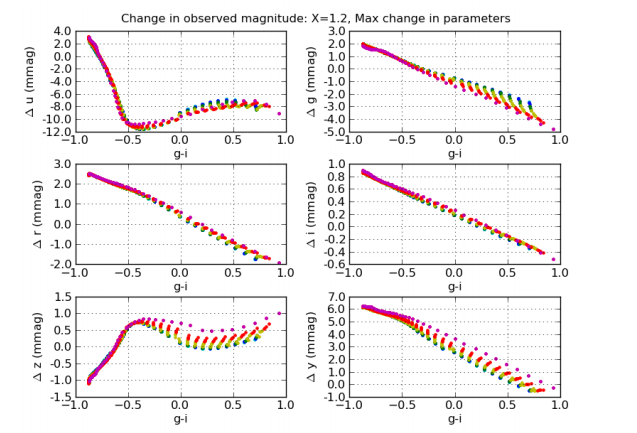
\includegraphics[width=14cm]{maxAtmosphereDeltas}
\end{center}
\caption{
  \label{figMaxAtmosphereDeltas}
  The change in the observed magnitude of stars in the temperature range 5000---35000K as the properties
  of the atmosphere are changed between two extreme models, keeping the airmass fixed at 1.2.  The different
  coloured points correspond to a range of metallicity and gravity.
  }
\end{figure}

To determine the optimal use of auxiliary data we need to see what can be learned directly from the
photometry and what information must come from elsewhere.

We will have many-colour photometry (\textit{ugrizy}) of \XXX{many, many} stars in each visit.  We know from
simulations of Kurucz models that as the properties of the atmosphere are varied there are several percent
level changes in fluxes, with percent-level scatter at a given $g - i$ colour (See figure
\ref{figMaxAtmosphereDeltas}).  It is not yet clear how much of this scatter can be regressed out using all
five available colours (see also section \ref{secSED}).

Even if the scatter can be removed to SRD precision (see appendix \ref{appSRD}), it is not clear how well
we will be able to characterize $S^{atm}$ across the filter $b$.

\subsection{Spatial Structure of the Atmosphere}

Even if the photometry is unable to constrain $S^{atm}$ well enough to satisfy the SRD requirements, it seems
very likely that we will be able to say something interesting.  Once we have implemented an initial version of
the photometric analysis we will be able to analyse wide-field camera data to explore the structure functions.
Obvious candidates are SDSS stripe82, DECam, and HSC.  These cameras have obvious tradeoffs in data
availability, available integration times, maximum scale probed and object density (and hence spatial
resolution).

\section{Flatfields}
\label{secFlatFielding}

Section \ref{secInstrumental} discusses analysing the response to the flatfield screen,
$(1 + i_b + \additive_b) \qe_b^{qe} \qe_b^{optics} \qe_b^{ccd}$.
Before we can create a flatfield image for band $b$ we need to:
\begin{itemize}
\item Decide what to do about $i_b(\lambda, \xb)$
\item Decide what to do about $\additive_b(\lambda, \xb)$
\item Decide what to do about $\qe_b^{optics}(\lambda, \xb)$
\item Decide what to do about $\qe_b^{ccd}(\lambda, \xb)$
\item Choose an SED
\end{itemize}

Correcting for $i$ is always desireable and we shall assume that it's been accomplished.\footnote{A better
  solution would be to design a flatfield screen which delivers $i \equiv 0$} It might seem obvious that the
flatfield should exclude $\additive$ and correct for $\qe^{optics} \qe^{ccd}$, resulting in a map of the
detector's true QE.  However, this is probably not a good idea as it
\begin{itemize}
\item leads to a complex background image
\item does not remove the need for sufficiently scrupulous algorithms to require access to the per-pixel
  geometrical information.
\end{itemize}

Once the data is warped to \eg a tangent plane these geometrical effects on QE are removed (the resampling
kernels include the determinant of the transformation's Jacobian).\footnote{ The inevitable distortion of the
  new projection will of course lead to a new $\qe^{optics}_b$.  } It would be possible to remove the effects
of the dimensions of individual pixels at the same time, but we shall choose to forgo this option; see the
discussion of background estimation in section \ref{secMeasuring}.

Removing $\additive_b$ from the flatfield also complicates the background, adding the scattered light and ghosting
back into the data.  As background estimation is already a challenging task (even with background matching),
this seems undesirable.

We therefore propose that the flatfields be calculated as follows:
\begin{itemize}
  \item Use the sky's SED. It would be possible to choose different sky models for different phases of the moon (or solar cycle), but this seems too complicated to be sensible.
  \item Do not correct for $\additive_b$ (resulting in an incorrect estimate of the sensitivity).
  \item Correct for $\qe_b^{qe}$
  \item Correct for $\qe_b^{optics}$
  \item Do not correct for $\qe_b^{ccd}$
\end{itemize}
This is the flatfield that best flattens the sky once warped onto a tangent plane,
at the cost of photometric errors.

We will further discuss the consequences of this choice in section \ref{secMeasuring}.

\subsection{Flatfields for Level 1}

This description is appropriate for level 2 processing, but level 1 is different and we must ensure that the
choices made during flatfield generation matches the adopted processing flow.  It may turn out that we need
different level 1 and level 2 flats.

\section{The object's SED}
\label{secSED}

Let us remember that we don't actually need to know the SED; we need merely to know enough about it to allow
us to make sufficiently accurate corrections from $C_{nat, b}$ to $C_{std, b}$.

We don't know our objects' SEDs, but we do know their multi-band fluxes $\{C_b\}$ and other parameters
$\theta$ (\eg morphological information).  There is a probability distribution $p(SED|\{C_b\}, \theta)$ which
may be compact, essentially reducing to a single reasonably well-defined SED, or may reflect the intrinsic
range of SEDs of objects with those properties.\footnote{
  In reality galaxies display colour gradients; we'll return to this in section \ref{secMeasuring}.
}

If we restrict our attention to stars, the colours probably determine the SED reasonably well (see
section \ref{secStellarPhotometry}).  Studies of galaxies photometric redshifts tell us that their SED is
often, but not always, reasonably well defined by the colours; QSOs show significant degeneracies, mostly
at redshifts below \c 2.5.

There is nothing we can do about this degeneracy, which means that we cannot hope to correctly estimate
$C_{std, b}$ for a subset of objects which we detect.  However, we will need to define a deterministic mapping
from colour to $\mbox{SED}(\{C_b\}, \theta)$ which will allow a consumer of the data to make their own
correction (see section \ref{secMeasuring}).

\section{Measuring the background level and $C_{std, b}$}
\label{secMeasuring}

\subsection{Background Subtraction}

We plan to background match exposures before sky subtraction, generating a stacked image in a sky projection.
This results in two data products:
\begin{itemize}
\item The background image in the stacked image $B^{stack}$.
\item The differences $B^i$ between this background image and the input images.
\end{itemize}
Because we measure $B^{stack}$ in sky coordinates the geometrical distortion terms $\qe_b^{optics}$ in
the flatfield illumination are automatically removed,\footnote{They are replaced by $\qe^{projection}$,
  but this term is not dependent on the boresights of the visits.}
and when we warp $B^i$ back to the corresponding
calibrated raw frame and subtract it we arrive at an image with $\qe_b^{optics}$ fully accounted for.

If we had included $\qe_b^{ccd}$ in the flatfield we would have handled the background correctly if we also
included it in the warps to and from sky coordinates, but we would not be able to forget about it as it
continues to have effects on the astrometry and photometry.\footnote{ it would also have made the warp code
  more complex and probably slower as the individual area of each pixel would have to be handled explicitly.
}

Having removed the background we can reconsider the choices we took when we built our flatfields
(section \ref{secFlatFielding}).
\begin{itemize}
  \item We no longer have any motivation to use the sky's SED, but do not know what to use instead.
  \item We should now correct the sensitivity for the effect of $\additive_b$ as it no longer complicates
    the sky subtraction.
  \item We could decide to now correct for $\qe_b^{ccd}$.
\end{itemize}

\subsection{Measuring $C_{std, b}$}

All photometric measurements can be thought of fitting a model $M$; $I = a M$.  Let us take this
model to describe the image above the atmosphere, and to be in photons not Joules.
We know our object's $(\{C_b\}, \theta)$, so we know which SED we should adopt (section \ref{secSED}).

The signal that we measure after (incorrectly) flat fielding with a flat constructed using the sky's SED is
$$
I_j = a \int_{b} \qe_{obj}^{atm} \frac{\qe_{j,obj}^{qe}}{\qe_{j,sky}^{qe}} \qe_j^{ccd} M_j P_b(\lambda)\, d\lambda + \epsilon_j
    \equiv a w_j + \epsilon_j
$$
where $I_j$ is the intensity of the $j^{th}$ pixel and $\epsilon_j$ the noise.  I'll drop the explicit
integral over filter $b$'s bandpass $P_b$ so all sensitivities in this section should be taken to be
bandpass-averaged.

If we take the $\epsilon_j$ to be independent Gaussians $N(0, \sigma_j^2)$, the maximum likelihood estimate
for the amplitude $a$ is
$$
a = \frac{\sum_j w_j I_j/\sigma_j^2}{\sum_j w_j^2/\sigma_j^2}
$$
and the total number of counts $C$ is $C = a\sum_j w_j$
(this is an unbiased estimate even if the errors aren't Gaussian).
It is almost always best
to set $\sigma^2_j = 1$ to avoid systematic errors as a function of magnitude, and we shall do so
in this discussion.

Let us assume that the ratio $\qe_{obj}^{qe}/\qe_{sky}^{qe}$ is constant for all the pixels in the
object.  This isn't necessary, we can handle it the same way as we'll handle $\qe_j^{qe}$, but it is probably
a good assumption and has some advantages.  In this case, we have
\begin{align*}
a =& \frac{1}{\qe_{obj}^{atm}} \frac{\qe_{sky}^{qe}}{\qe_{obj}^{qe}}
                         \frac{\sum_j (\qe_j^{ccd} M_j) I_j}{\sum_j (\qe_j^{ccd} M_j)^2}\\
C =& a \sum_j \qe_j^{ccd} M_j\\
\noalign{and, correcting to a standard atmosphere, and writing $w = \qe_j^{ccd} M_j$}
C_{std} =& \frac{\qe_{obj,std}^{atm}}{\qe_{obj}^{atm}} \frac{\qe_{sky}^{qe}}{\qe_{obj}^{qe}}
                         \, \frac{\sum_j w_j I_j  \sum_j w_j}{\sum_j (w_j)^2} \\
   \equiv& \frac{\qe_{obj,std}^{atm}}{\qe_{obj}^{atm}} \frac{\qe_{sky}^{qe}}{\qe_{obj}^{qe}}
                         \, C_{raw}
\end{align*}

\newcommand{\cSED}{c_{\scriptscriptstyle\rm SED}}

If we have $n$ exposures this generalises to
\begin{align*}
C_{std}  =& \sum_r
  \frac{\qe_{obj,std}^{atm}}{\qe_{obj}^{atm,r}} \frac{\qe_{sky}^{qe,r}}{\qe_{obj}^{qe,r}} \, C_{raw}^r\\
 \equiv& \sum_r \cSED^r C_{raw}^r
\end{align*}
I have kept the per-visit suffix $r$ in the $\qe^{qe}$ to allow for different CCDs in the focal
plane having different sensitivities, and for radial variation in the filter properties.

Note that the SED doesn't enter into the pixel-dependent part, $C_{raw}^r$, making it relatively simple to
adopt a different SED and recalculate $C_{std}$ if we know the $\cSED^r$.  We don't need to save $\cSED^r$
for every object as we only need the SED, and that is known given $(\{C_b\}, \theta)$.  This simplification
depends on our assumption about the constancy of $\qe_{obj}^{qe}/\qe_{sky}^{qe}$ over the object.

\subsection{Colour Gradients}

Because we using a model-based approach to handle SED dependencies we can easily handle more complicated
problems; for example, if we are using a bulge/disk decomposition we are estimating the colours of each
component, and can handle their SEDs separately when fitting our model.

\appendix

\section{Science Requirements Document (SRD)}
\label{appSRD}

The SRD specifications are:

\begin{description}
\item{Repeatability}\\
  the median value of the photometric scatter for each star (the rms of calibrated
  magnitude measurements around the mean calibrated magnitude) shall not exceed 5 millimags in gri, 7.5
  millimags in uzy. No more than 10\% of these objects should have a photometric scatter larger than 15 mmag
  in gri, 22.5 mmag in uzy. This requirement sets the level above which we can reliably detect intrinsic
  variability in a single source.
  
\item{Uniformity}\\
  the rms of the internal photometric zeropoint error (for each visit) shall not exceed 10
  millimags in grizy, 20 millimags in uzy. No more than 10\% of these sources can be more than 15 mmag in gri
  or 22.5 mmag in uzy from the mean internal zeropoint. This places a constraint on the stability of the
  photometric system across the sky as well as an upper limit on various systematic uncertainties, such as any
  correlation of photometric calibration with varying stellar populations (or colors). This makes the
  photometry of sources directly comparable over the entire sky, and when combined with the previous
  requirement, creates a stable photometric system across the sky and over time, in a single filter.

\item{Band-to-band photometric calibration}\\
  The absolute band-to-band zeropoint calibration for main sequence
  stars must be known with an rms accuracy of 5 millimags for any color not involving u band, 10 millimags for
  colors constructed with u band photometry. This requirement ties photometric measurements in different
  filters together, enabling precise measurement of colors, and allows LSST photometry to be compared with
  that from other optical telescopes, and with astrophysical models.

\item{Absolute photometric calibration}\\
  The LSST photometric system must transform to an external physical
  scale (\eg AB mags) with an rms accuracy of 10 millimags. This is essential for comparing with photometry
  from other wavelength regions, such as IR or UV.
\end{description}

\section{Glossary}

\begin{description}
  \item{DN}\\
    Data Number; the value of a pixel as read from the detector (also called ADU)
  \item $\screen$\\
    The illumination of the focal plane due to the flatfield screen.
  \item{ISR}\\
    Instrumental Signature Removal (remove bias, flatfield, \etc)
  \item{QE}\\
    Quantum Efficiency
  \item $\Flat$\\
    The image of the flatfield screen in the $b$ band.
  \item $\qe$
    The quantum efficiency of a pixel.
    \begin{description}
    \item $\qe_b^{qe}$
      The probability of a photon reaching the detector multiplied by the probability
      of its being absorbed (but neglecting vignetting)
    \item $\qe_b^{vig}$
      The probability that a photon will not be vignetted
    \item $\qe_b^{optics}$
      The effective area of a pixel (in units of nominal pixels) allowing for distortions
    \item $\qe_b^{ccd}$
      The effective area of a pixel (in units of nominal pixels) allowing for physical changes
      in the size of the pixel (\eg `ragged gates').
    \end{description}    

  \item $S^{atm}$\\
    The probability that a photon will pass through the atmosphere for a given visit.
  \item $S_b^{sys}$\\
    The probability that a photon will pass through the telescope and camera (with the $b$ filter)
    and be absorbed by the detector;  assumed to vary relatively slowly with time.
  \item $S_{b, std}$\\

    The probability that a photon incident on the atmosphere will be detected under `standard' conditions; all
    photometry is referred to this probability.

  \item{SED}\\
    Spectral Energy Distribution
  \item{S/N}\\
    Signal-to-noise ratio
  \item{SRD}\\
    Science Requirements Document
  \item{TBD}\\
    The meaning of this acronym is To Be Decided
\end{description}

\end{document}
